\begin{frame}{Intégration avec ROCK2}{Contribution 3 | Étude numérique, diffusion et MRA}

    \begin{textblock*}{40pt}(0.1\paperwidth,0.87\paperheight)
        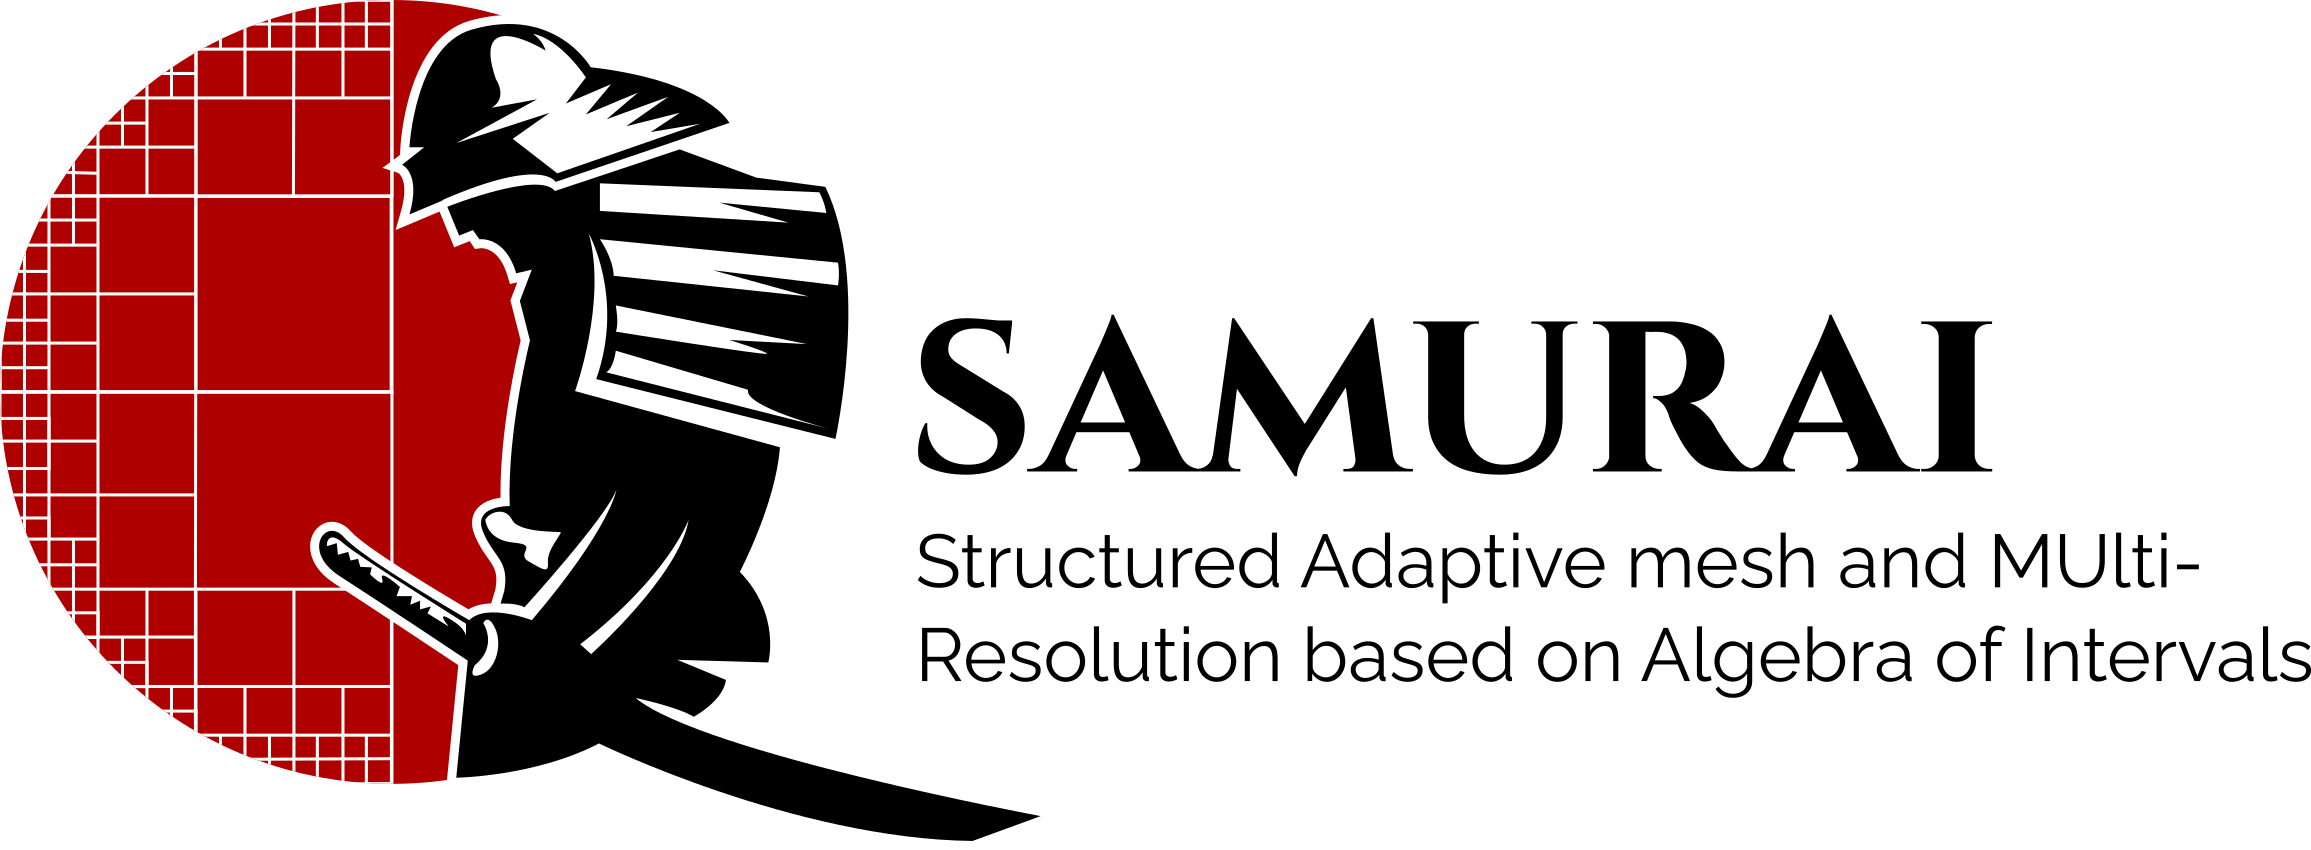
\includegraphics[scale=.03]{medias/2_/1_/light_logo.png}
    \end{textblock*}
    \centering
    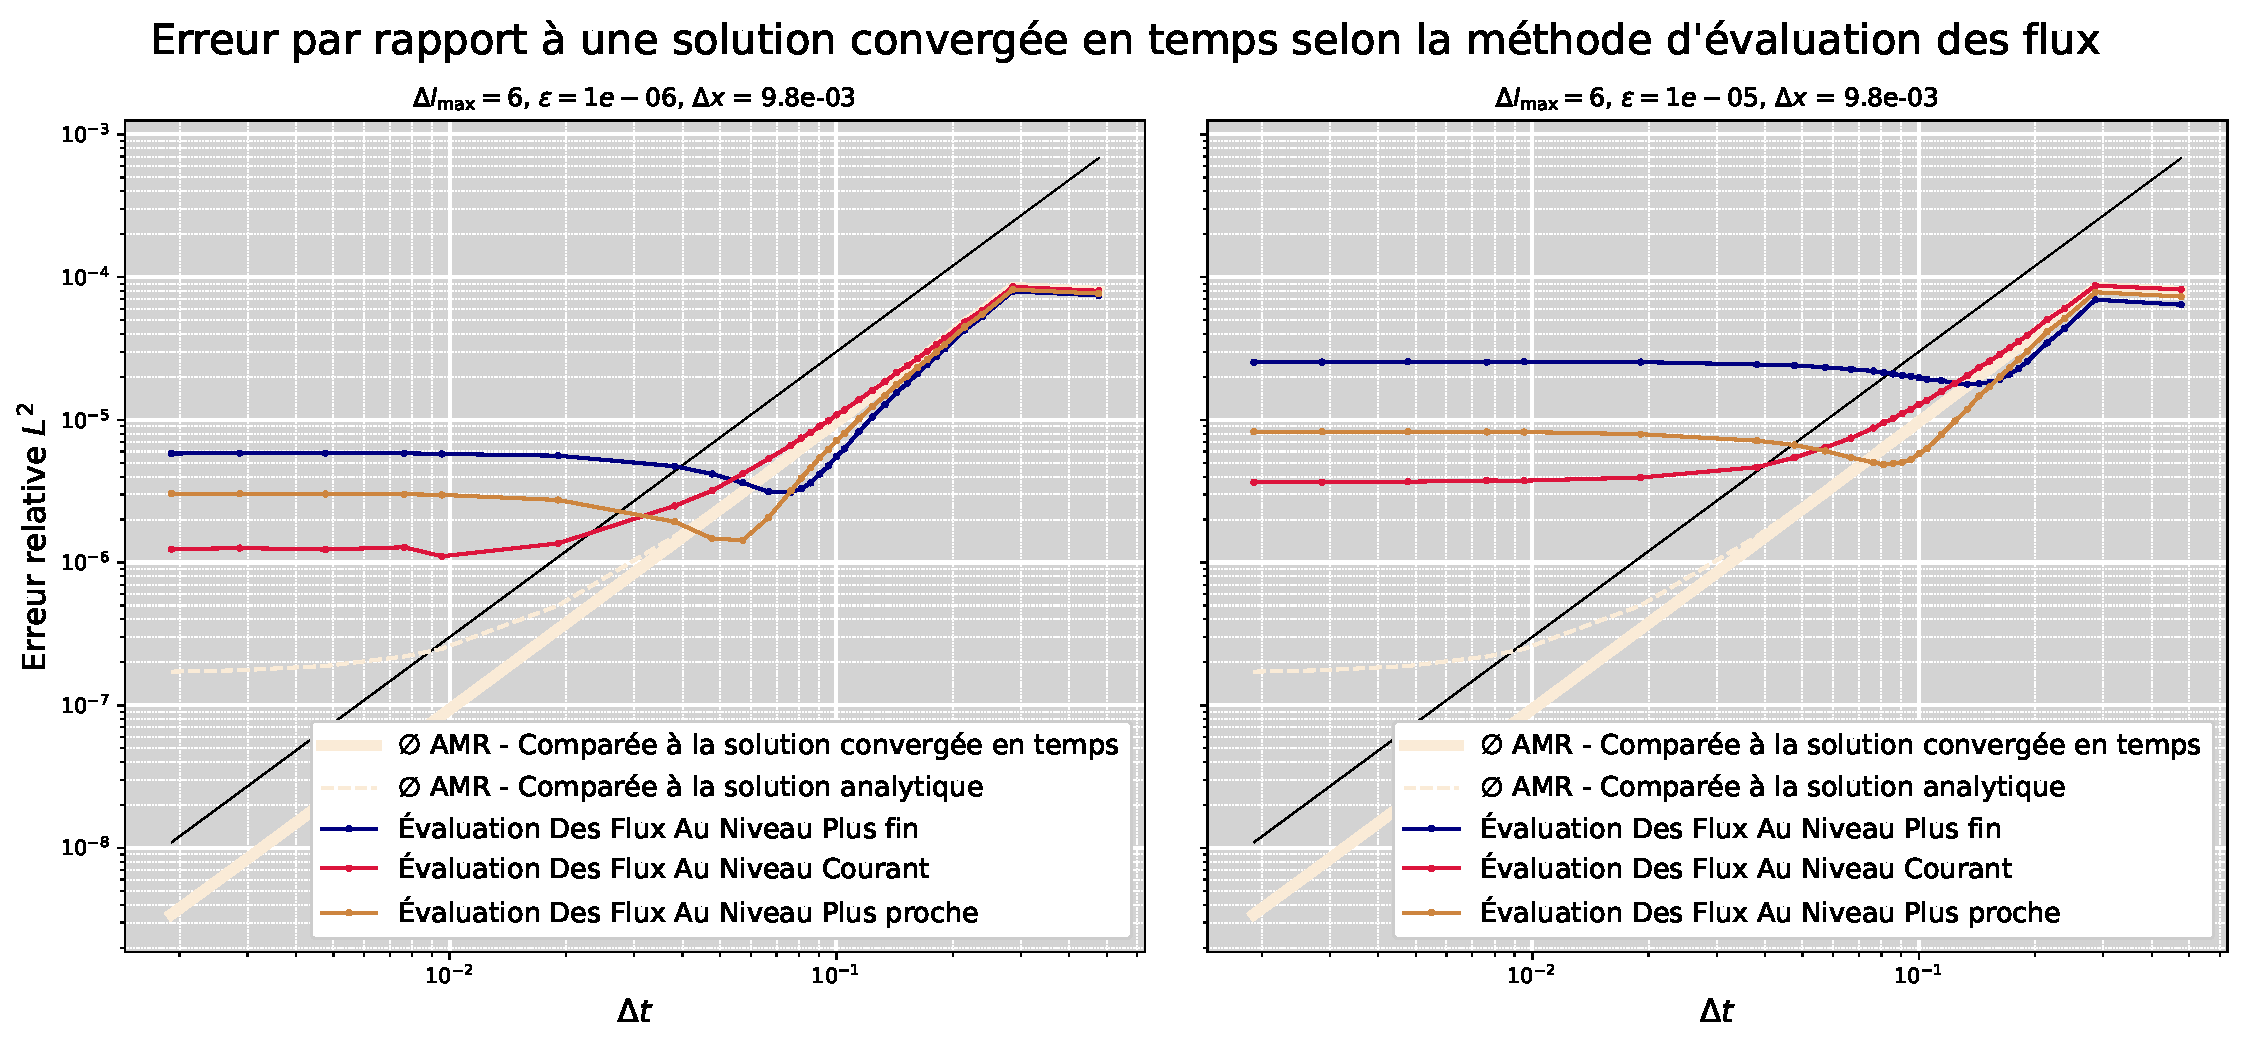
\includegraphics[width= .9\textwidth]{medias/2_/3_/flux_reconstruction_method_diffusion.pdf}
        \visible<2->{\scriptsize{\vspace{-1.75em}\begin{align}\label{eq:equiv_cfl_recons}
            \frac{\partial u}{\partial t}
            =&+ D \frac{\partial^{2}u}{\partial x^{2}}
            + \Delta x^{2}\, D \, \Bigl( 
            \frac{\lambda}{2} (2^{2 \Delta l} - 1) + \frac{2^{2 \Delta l} }{12} (1 - 3 \Delta l)
            \Bigr)\frac{\partial^{4}u}{\partial x^{4}}\
            - \Delta x^{4} \frac{D \lambda^{2} \frac{\partial^{6}u}{\partial x^{6}}}{6} - \Delta x^{6} \frac{D \lambda^{3} \frac{\partial^{8}u}{\partial x^{8}}}{24}
            + \mathcal{O}(\Delta x^7). 
        \end{align}}}
    \begin{textblock*}{40pt}(0.2\paperwidth,0.96\paperheight)
        {\color{black}{+ Ponio}}
    \end{textblock*}
    \href{https://github.com/Ocelot-Pale/etude_MR_RK2}{\color{Primary} \underline{Visualisation de la distribution des erreurs.}}\color{black}
\end{frame}
